\documentclass{article}
\usepackage{graphicx} %package to manage images
\graphicspath{ {./figures/} }
\usepackage{hyperref}
\usepackage{caption}
\usepackage[font=scriptsize]{subcaption}
\captionsetup[figure]{labelsep=none}
\captionsetup[table]{labelsep=none}
\usepackage{bbm}
\usepackage{amsmath}
\usepackage{import}
\usepackage{array}
\usepackage{booktabs}
\usepackage{afterpage}
\usepackage{floatrow}
\usepackage{pdflscape}
\usepackage{soul}
\usepackage{float}
\usepackage{adjustbox}
\usepackage{longtable}


\title{trends in health in pregnancy (overleaf)}

\date{April 2025}

\begin{document}

\maketitle

TODO
- add short note after each figure/table and about how it was generated

\section{CDF of pre-pregnancy BMI}

\begin{figure}[H]
    \centering
    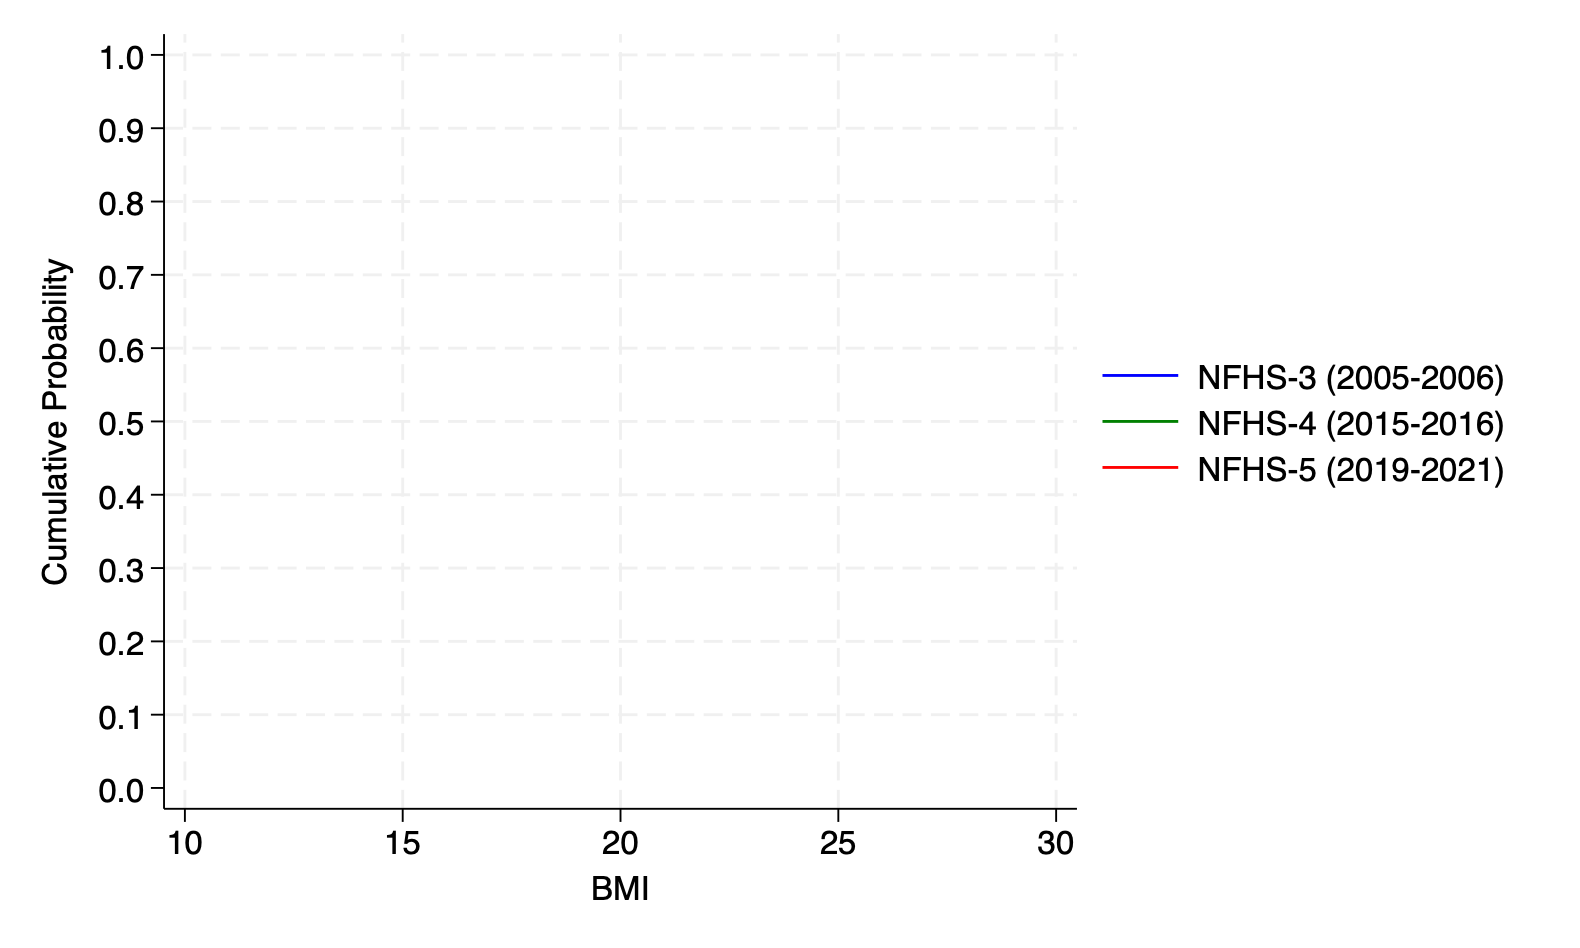
\includegraphics[width=\textwidth]{figures/cdf prepregnancy bmi.png}
    \caption{: CDFs of Estimated Pre-Pregnancy BMI in NFHS 3, 4, \& 5}
    
\end{figure}

The whole distribution of BMI for pre-pregnant women is increasing in subsequent survey rounds. 

Generated cdf using cumul command with pre-pregnancy weights. I am not sure if \textbf{I need to normalize these since I am stacking survey rounds?}

\section{CDF of 9+ mo pregnant BMI}

\begin{figure}[H]
    \centering
    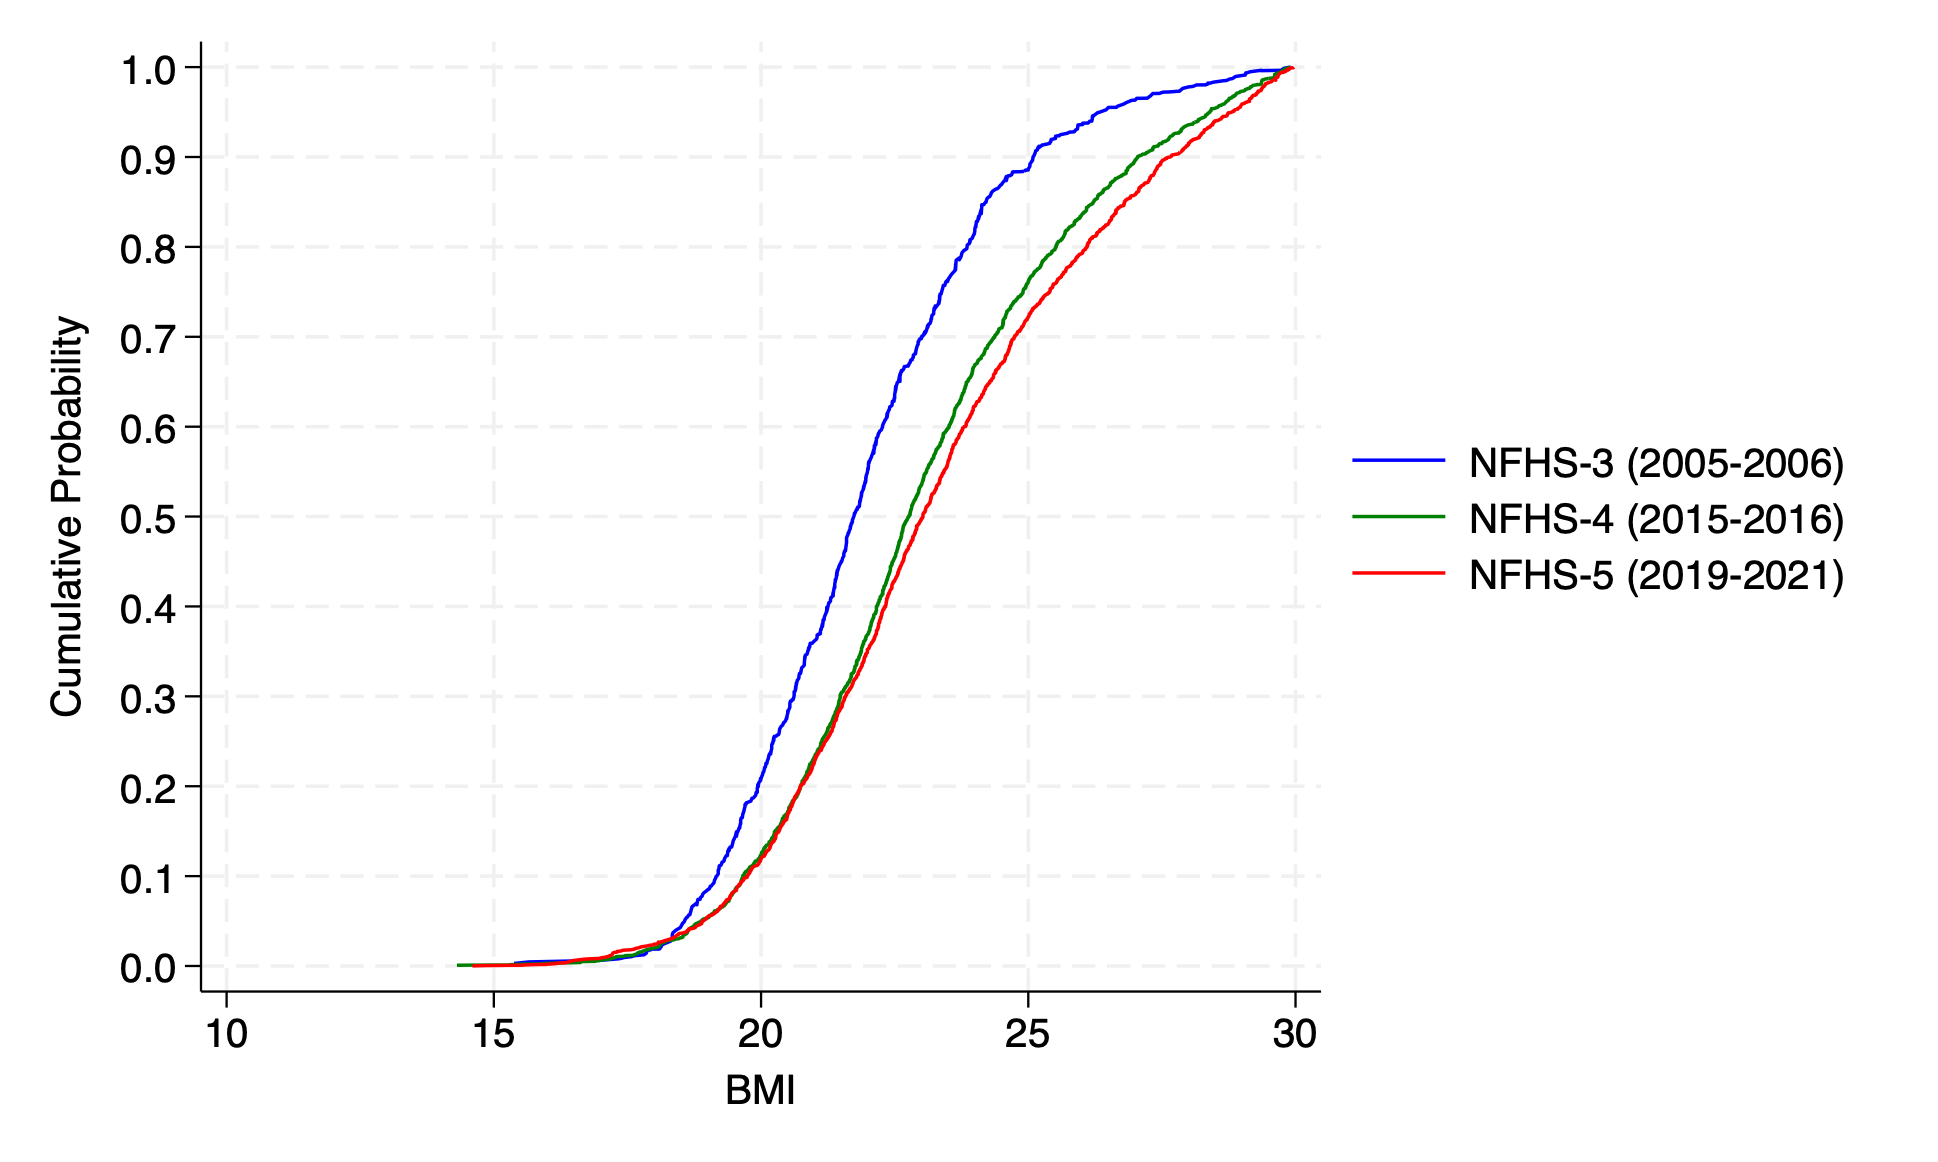
\includegraphics[width=\textwidth]{figures/cdf nine months bmi.png}
    \caption{: CDFs of Observed BMI at 9+ months pregnant in NFHS 3, 4, \& 5}
    
\end{figure}

The whole distribution of BMI for 9+ mo pregnant women is increasing in subsequent survey rounds. \textbf{Should I just use v005, within survey round weights?}

Also, the curves are about equally shifted right relative to the pre-pregnant curves in all survey rounds. 

Generated cdf using cumul command with aweights normalized across all survey rounds.

\section{CDF and boxplot of age}

\begin{figure}[H]
    \centering
    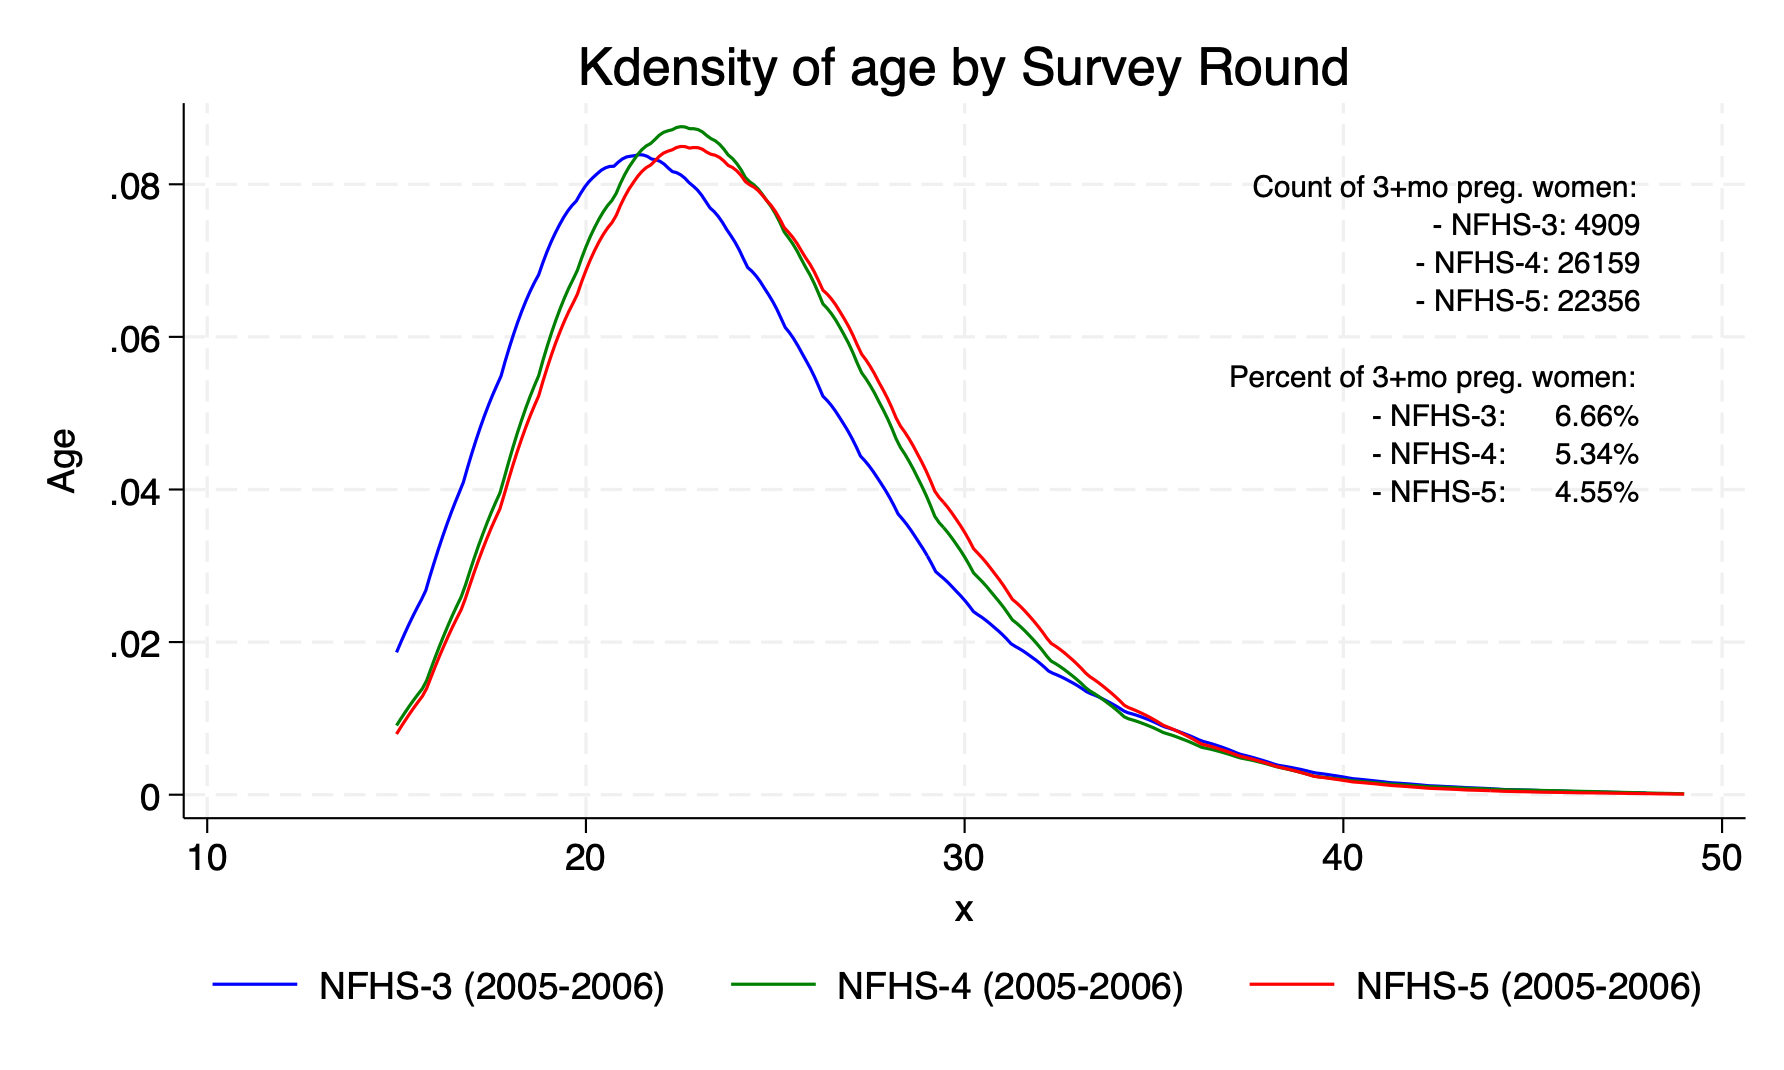
\includegraphics[width=\textwidth]{figures/kdensities ages.png}
    \caption{: Kernel density of the ages of currently pregnant women in NFHS 3, 4, \& 5}
\end{figure}

The age distribution of currently pregnant women is increasing. Between NFHS-4 and NFHS-5, it seems like it is moreso widening - the peak is only barely shifting right. 

\begin{figure}[H]
    \centering
    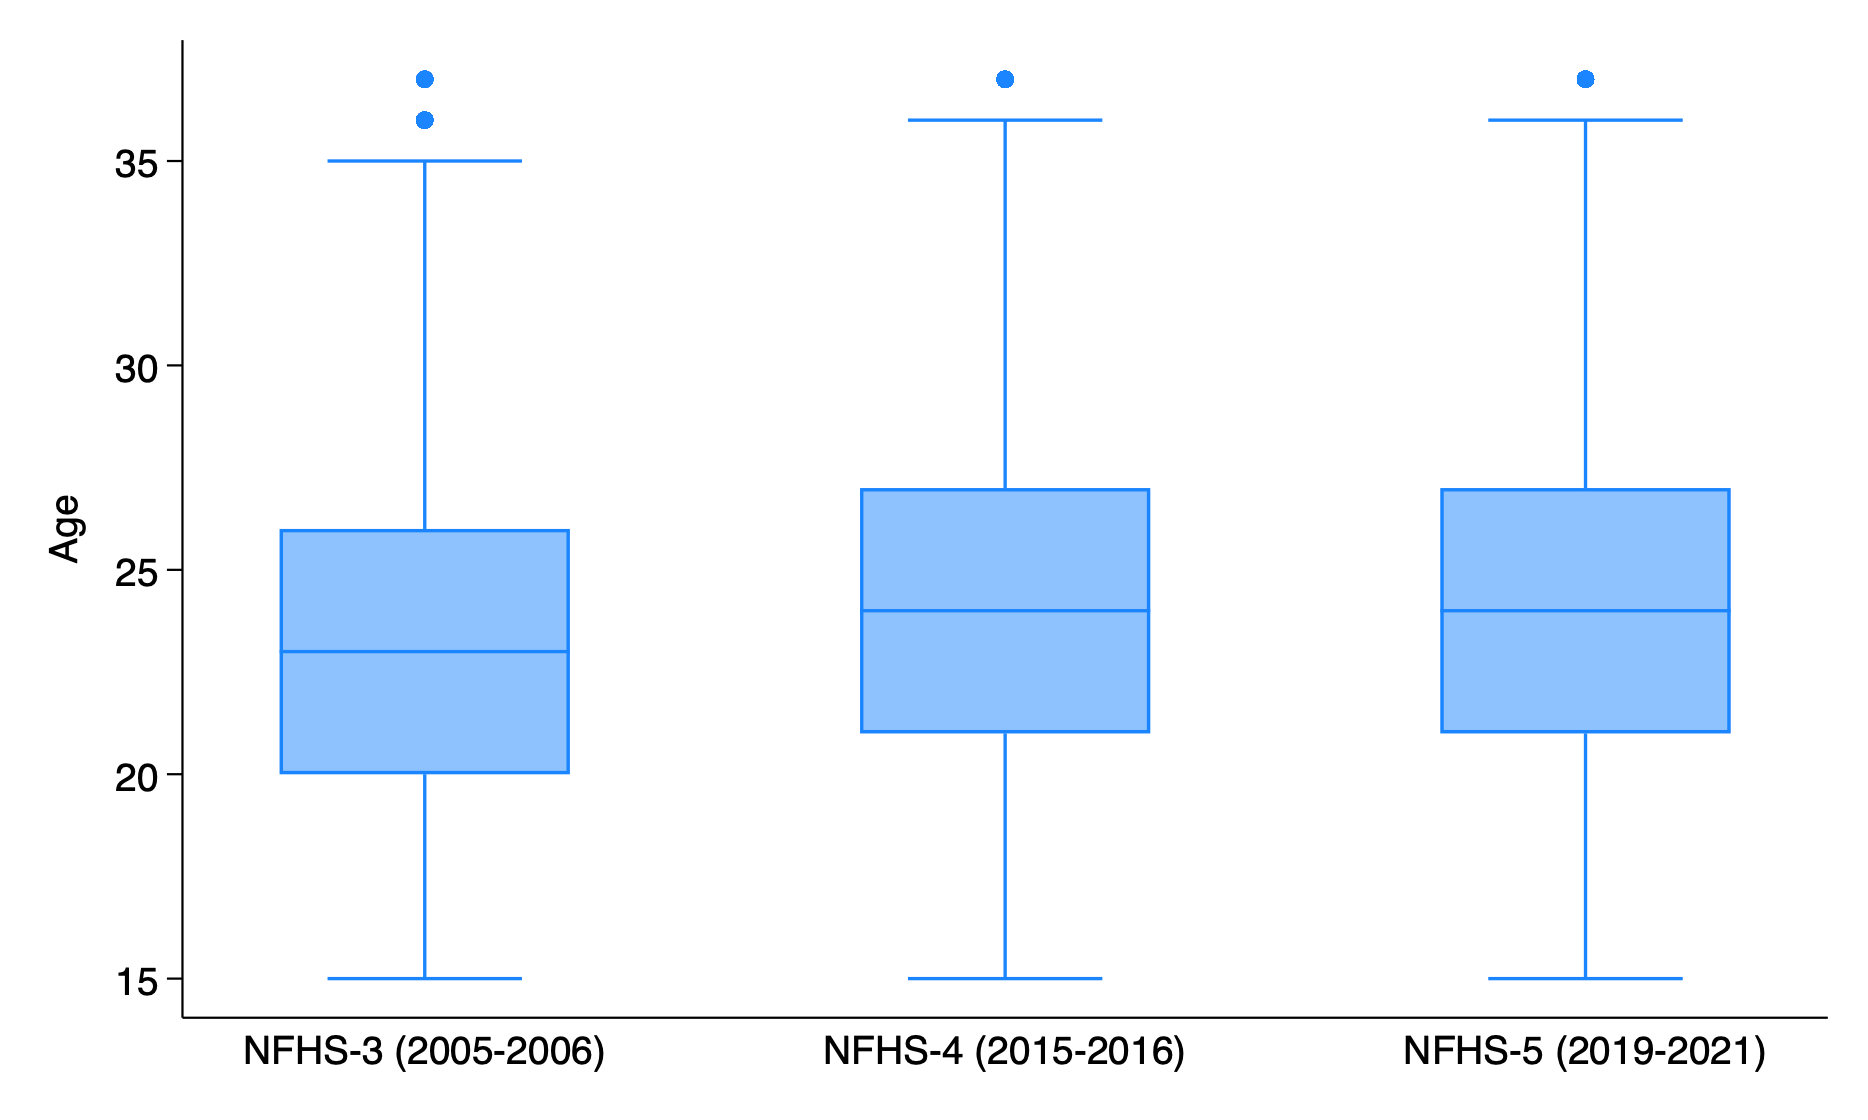
\includegraphics[width=\textwidth]{figures/boxplots ages.png}
    \caption{: Box plots of the age distributions of currently pregnant women NFHS 3, 4, \& 5}
\end{figure}

In this figure, it looks like there's less of a change at all in the age distribution of currently pregnant women between NFHS-4 and NFHS-5. 

Just used graph box with aweights normalized across survey rounds. 

\section{Bar graph of parity}

\begin{figure}[H]
    \centering
    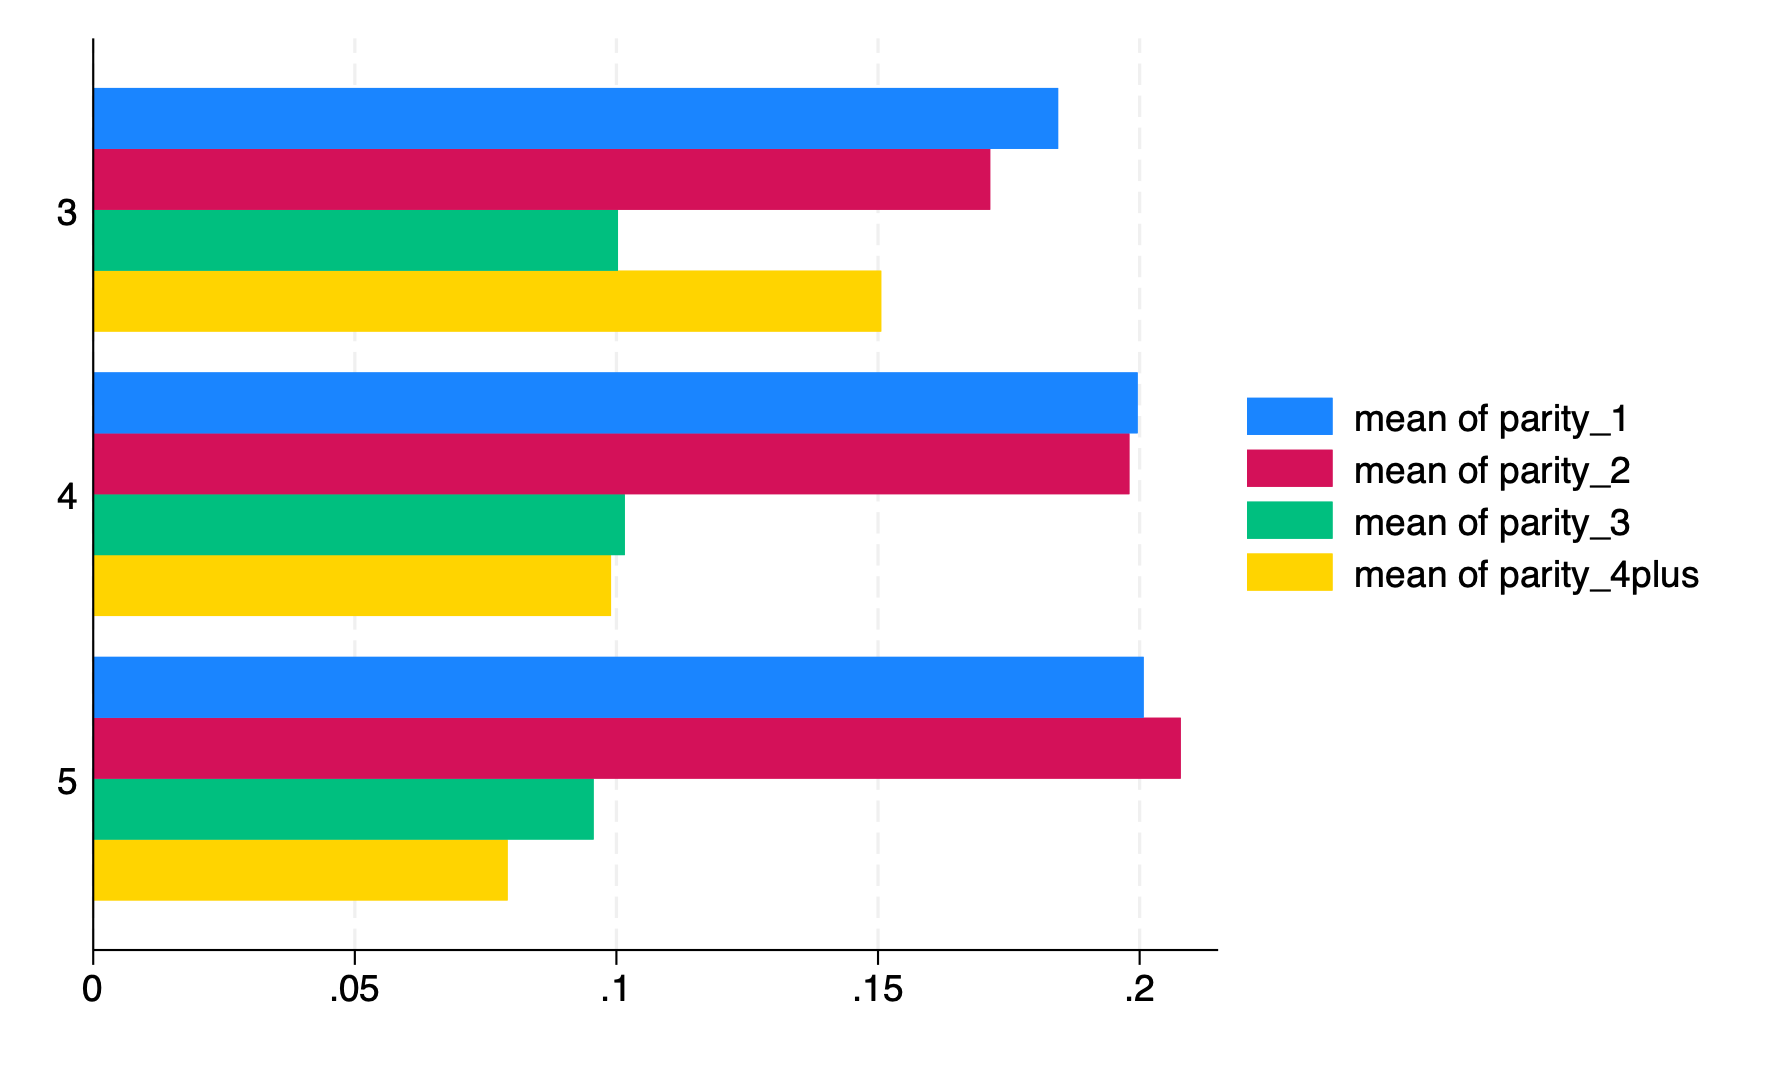
\includegraphics[width=\textwidth]{figures/bar graph number of children.png}
    \caption{: Bar graph of number of living children among currently pregnant women in the NFHS 3, 4, \& 5}
\end{figure}

Less women are giving birth at higher parities - largely parity 4+, and there is less change happening at just parity 3. But significantly more births are happening at parities 1 and 2.

Generated using hbar and v005 aweights - within survey round.

\section{Distribution of gestational duration}

\begin{table}[H]
    \centering
    \caption{: Proportion of pregnant women by gestational duration in the NFHS 3, 4, \& 5}
    \label{tab:sumstat}
    \adjustbox{width=\textwidth}{\begin{tabular}{l*{6}{c}}
\toprule
            &NFHS-3 (2005-2006)&            &NFHS-4 (2015-2016)&            &NFHS-5 (2019-2021)&            \\
            &\multicolumn{1}{c}{Mopreg}&\multicolumn{1}{c}{Moperiod}&\multicolumn{1}{c}{Mopreg}&\multicolumn{1}{c}{Moperiod}&\multicolumn{1}{c}{Mopreg}&\multicolumn{1}{c}{Moperiod}\\
\midrule
\midrule
1           &       1.807&       5.163&       4.602&       1.762&       4.987&       4.473\\
2           &       8.775&       8.199&       8.635&       8.696&       7.657&       8.285\\
3           &       13.44&       13.26&       12.38&       13.14&       12.51&       11.98\\
4           &       12.85&       12.83&       12.75&       12.74&       11.96&       12.37\\
5           &       12.73&       13.42&       12.21&       12.57&       12.60&       11.80\\
6           &       12.10&       12.19&       12.42&       11.86&       11.48&       11.82\\
7           &       11.84&       11.92&       12.00&       11.68&       11.20&       11.50\\
8           &       12.33&       12.02&       13.07&       12.14&       11.20&       12.26\\
9           &       11.28&       8.505&       9.477&       10.93&       7.918&       8.995\\
10          &       2.651&       2.060&       2.165&       2.638&       2.052&       2.144\\
11          &       0.196&       0.436&       0.277&       0.196&       0.436&       0.277\\
\bottomrule
\multicolumn{7}{l}{\footnotesize Mopreg refers to respondents self reported gestational duration. Moperiod refers months since last menstrual period.}\\
\end{tabular}
}
\end{table}

Women reporting they're currently pregnant at 1mo is decreasing after NFHS-4? 
Doesn't seem like there's much of a pattern in the discrepancies?
Decline at 9 months - maybe due to an increase in induced pregnancies?

Generated using the sum command with v005 aweights - within survey round.

\section{Wanted pregnancies}

\begin{table}[H]
    \centering
    \caption{: Proportion of wanted pregnancies among pregnant women by parity in the NFHS 3, 4, \& 5}
    \label{tab:sumstat}
    \adjustbox{width=\textwidth}{{
\def\sym#1{\ifmmode^{#1}\else\(^{#1}\)\fi}
\begin{tabular}{l*{3}{c}}
\hline\hline
            &\multicolumn{1}{c}{NFHS-3}&\multicolumn{1}{c}{NFHS-4}&\multicolumn{1}{c}{NFHS-5}\\
\hline
\hline
Parity 1    &       85.14         &       94.99         &       94.85         \\
Parity 2    &       74.04         &       88.12         &       88.97         \\
Parity 3    &       71.06         &       80.72         &       81.92         \\
Parity 4+   &       55.21         &       69.60         &       74.63         \\
\hline\hline
\multicolumn{4}{l}{\footnotesize \textit{t} statistics in parentheses}\\
\multicolumn{4}{l}{\footnotesize \sym{*} \(p<0.05\), \sym{**} \(p<0.01\), \sym{***} \(p<0.001\)}\\
\end{tabular}
}
}
\end{table}

More women report they wanted their current pregnancy at all parities. 

Generated using sum command and v005 aweights within survey round. 

\section{Modern contraception}

\begin{table}[H]
    \centering
    \caption{: Proportion of married non-pregnant women using modern contraception in the NFHS 3, 4, \& 5}
    \label{tab:sumstat}
    \adjustbox{width=\textwidth}{\begin{tabular}{l*{3}{c}}
\toprule
            &\multicolumn{1}{c}{NFHS-3 (2005–2006)}&\multicolumn{1}{c}{NFHS-4 (2015–2016)}&\multicolumn{1}{c}{NFHS-5 (2019–2021)}\\
\midrule
\midrule
No living boy child&       12.06&       15.33&       25.50\\
No children &       4.031&       6.664&       14.29\\
\bottomrule
\end{tabular}
}
\end{table}

More women are using modern contraception regardless of their birth history/ sex ratio.

Modern method defined according to the reweighting code. Generated using sum command and v005 aweights within survey round. 

\section{Ultrasound}

\begin{figure}[H]
    \centering
    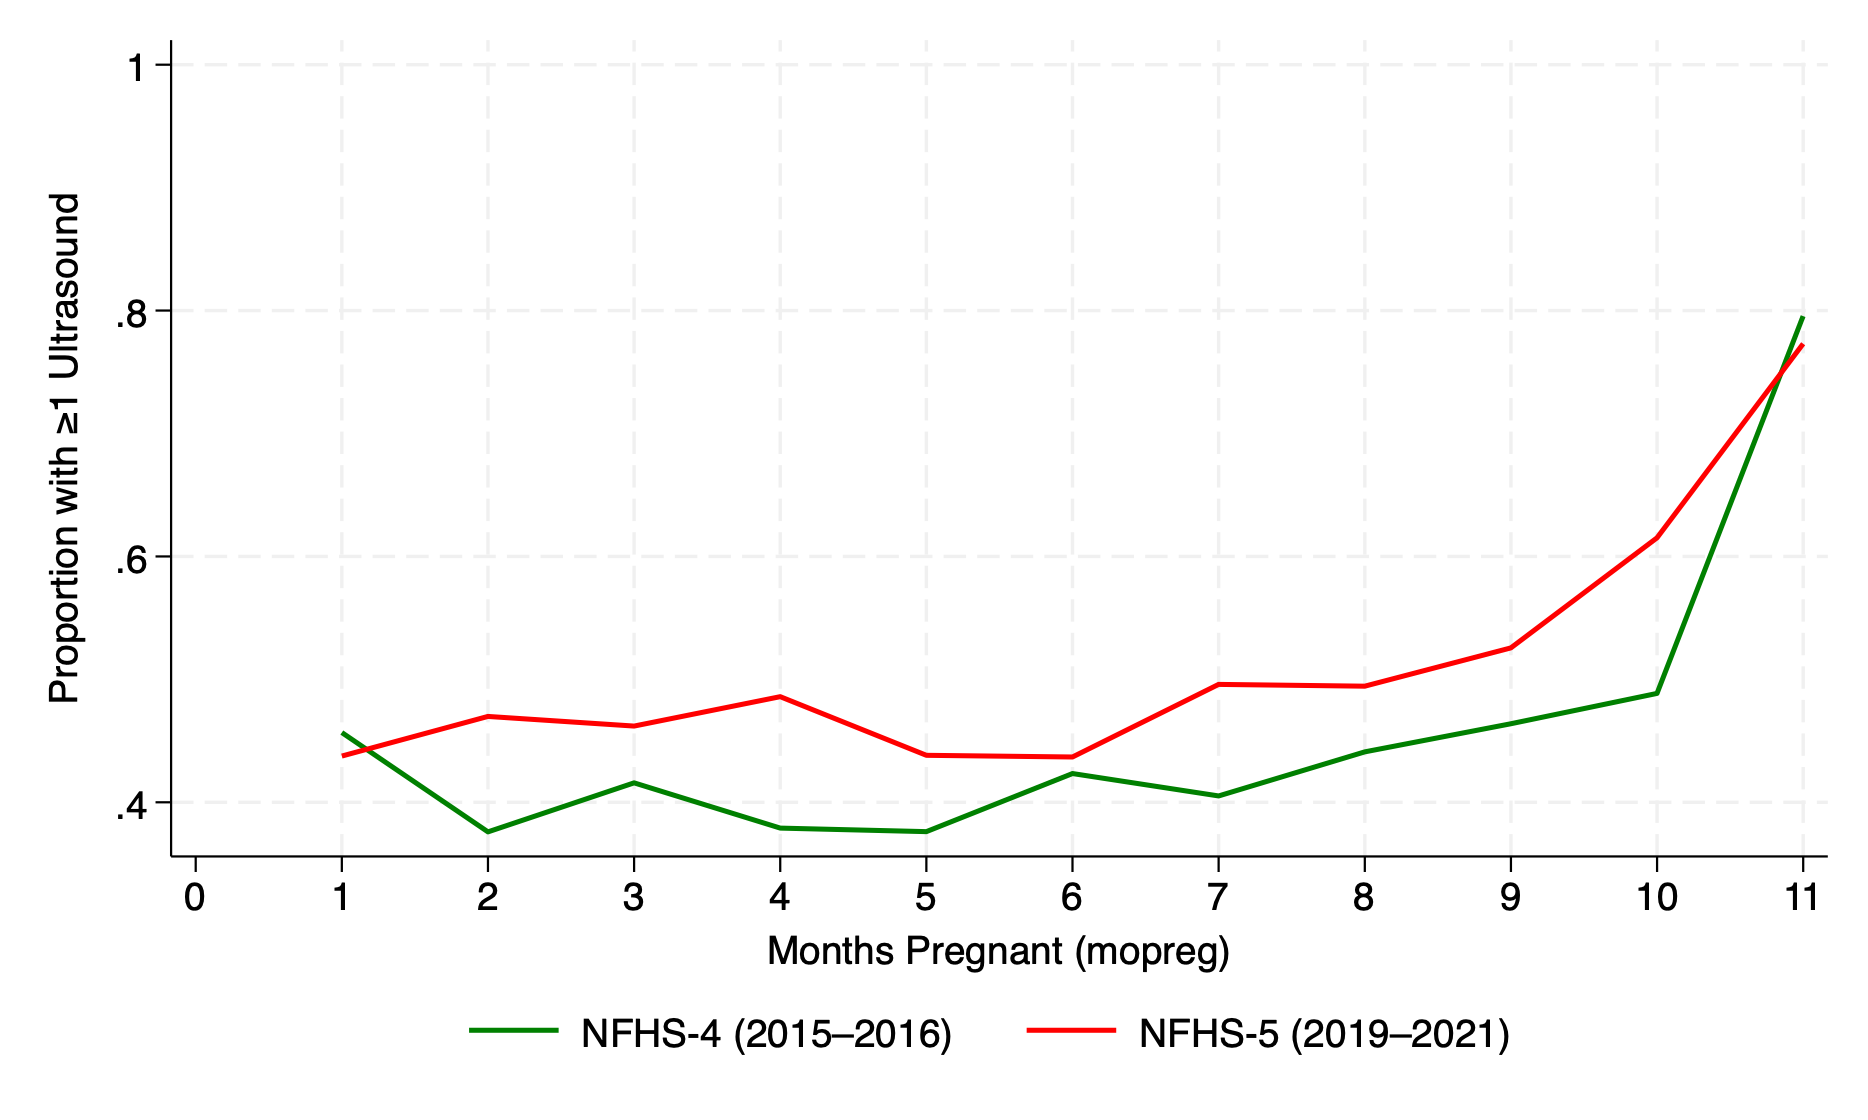
\includegraphics[width=\textwidth]{figures/ultrasound by pregnancy duration.png}
    \caption{: Proportion of pregnant women who have had an ultrasound by gestational duration in NFHS 4, \& 5}
\end{figure}

Women are having ultrasounds earlier during pregnancy. Also, the proportion of women having ultrasounds at all is about the same.

Generated using s236 "Ultrasound at any time".
Collapsed the data to mopreg round using v005 aweights. 
Then I calculated total with ultrasound/ full total at each mopreg round.

\section{Pregnancy reporting}

\begin{table}[H]
    \centering
    \caption{: Proportion of women who report not being pregnant by months since last period in the NFHS 3, 4, \& 5}
    \label{tab:sumstat}
    \adjustbox{width=\textwidth}{\begin{tabular}{l*{3}{c}}
\toprule
            &\multicolumn{1}{c}{NFHS-3}&\multicolumn{1}{c}{NFHS-4}&\multicolumn{1}{c}{NFHS-5}\\
\midrule
\midrule
1           &       99.83&       99.60&       99.71\\
2           &       73.45&       75.11&       75.44\\
3           &       43.89&       59.74&       60.68\\
4           &       20.38&       34.09&       33.83\\
5           &       14.19&       23.30&       22.94\\
6           &       14.26&       23.54&       23.86\\
7           &       6.679&       15.51&       16.26\\
8           &       6.748&       16.39&       13.93\\
9           &       7.396&       22.42&       25.14\\
10          &       43.12&       65.42&       68.42\\
11          &       85.99&       84.25&       91.11\\
\bottomrule
\end{tabular}
}
\end{table}


TODO: interpret 
is there something wrong at moperiod=11?
Generated by using sum command on v213==0 using v005 aweights at moperiod as calculated in the reweighting file. 


\section{Sample size}

\begin{table}[H]
    \centering
    \setlength{\tabcolsep}{4pt} % shrink column padding
    \footnotesize % shrink text
    \caption{: Sample sizes table}
    \label{tab:sumstat}
    \begin{adjustbox}{width=\textwidth}
        {
\def\sym#1{\ifmmode^{#1}\else\(^{#1}\)\fi}
\begin{tabular}{l*{3}{c}}
\toprule
                    &      NFHS-3&      NFHS-4&      NFHS-5\\
                    &\multicolumn{1}{c}{}&\multicolumn{1}{c}{}&\multicolumn{1}{c}{}\\
                    &           N&           N&           N\\
\midrule
india               &        5242&       27867&       24582\\
focus               &         976&        7590&        5647\\
central             &         496&        3719&        2581\\
east                &         561&        2698&        2388\\
west                &         558&        1817&        2040\\
north               &         801&        3416&        4356\\
south               &         742&        2513&        2893\\
northeast           &         813&        3925&        3301\\
rural               &        3239&       21192&       19772\\
urban               &        2003&        6675&        4810\\
forward             &        1011&        3219&        2496\\
obc                 &        1364&        8821&        7456\\
dalit               &         858&        4840&        4336\\
adivasi             &         354&        2774&        2631\\
muslim              &         920&        4494&        3968\\
sikh\_jain\_christian &         536&        2706&        2557\\
Observed in nuclear &        2057&        8700&        7293\\
Observed in sasural &        2439&       15001&       13680\\
Observed in meika   &         585&        3400&        2966\\
other               &          98&         458&         429\\
\midrule
Observations        &        5242&       27867&       24582\\
\bottomrule
\end{tabular}
}

    \end{adjustbox}
\end{table}



\begin{table}[H]
    \centering
    \setlength{\tabcolsep}{4pt} % shrink column padding
    \footnotesize % shrink text
    \caption{: Sample sizes table}
    \label{tab:sumstat}
    \begin{adjustbox}{width=\textwidth}
        {
\def\sym#1{\ifmmode^{#1}\else\(^{#1}\)\fi}
\begin{tabular}{l*{3}{ccc}}
\hline\hline
                    &      NFHS-3&            &            &      NFHS-4&            &            &      NFHS-5&            &            \\
                    &\multicolumn{3}{c}{}                  &\multicolumn{3}{c}{}                  &\multicolumn{3}{c}{}                  \\
                    &        Mean&          lb&          ub&        Mean&          lb&          ub&        Mean&          lb&          ub\\
\hline
eag                 &        0.56&      0.5450&      0.5704&        0.53&      0.5279&      0.5388&        0.54&      0.5297&      0.5413\\
north               &        0.12&      0.1164&      0.1333&        0.11&      0.1094&      0.1163&        0.13&      0.1300&      0.1380\\
central             &        0.28&      0.2733&      0.2964&        0.28&      0.2786&      0.2884&        0.27&      0.2621&      0.2724\\
east                &        0.27&      0.2613&      0.2841&        0.25&      0.2485&      0.2580&        0.27&      0.2631&      0.2734\\
northeast           &        0.04&      0.0329&      0.0427&        0.03&      0.0306&      0.0344&        0.04&      0.0393&      0.0440\\
Rural               &        0.75&      0.7410&      0.7631&        0.71&      0.7099&      0.7198&        0.74&      0.7389&      0.7491\\
Urban               &        0.25&      0.2369&      0.2590&        0.29&      0.2802&      0.2901&        0.26&      0.2509&      0.2611\\
Forward Caste       &        0.26&      0.2445&      0.2668&        0.20&      0.1915&      0.2002&        0.17&      0.1690&      0.1778\\
OBC                 &        0.42&      0.4040&      0.4292&        0.45&      0.4445&      0.4553&        0.44&      0.4356&      0.4472\\
Dalit               &        0.20&      0.1912&      0.2117&        0.22&      0.2125&      0.2214&        0.23&      0.2234&      0.2331\\
Adivasi             &        0.09&      0.0848&      0.0996&        0.10&      0.0924&      0.0988&        0.10&      0.0968&      0.1038\\
Muslim              &        0.18&      0.1691&      0.1887&        0.17&      0.1692&      0.1775&        0.17&      0.1686&      0.1774\\
Sikh/Jain/Christian &        0.03&      0.0260&      0.0347&        0.04&      0.0339&      0.0379&        0.03&      0.0321&      0.0364\\
Observed in nuclear family&        0.36&      0.3499&      0.3745&        0.29&      0.2831&      0.2930&        0.27&      0.2617&      0.2720\\
Observed in sasural &        0.45&      0.4336&      0.4590&        0.53&      0.5244&      0.5352&        0.55&      0.5472&      0.5588\\
Observed in meika   &        0.12&      0.1158&      0.1327&        0.13&      0.1225&      0.1297&        0.13&      0.1261&      0.1339\\
Observed in mother-in-law's home&        0.13&      0.1245&      0.1419&        0.16&      0.1511&      0.1590&        0.16&      0.1554&      0.1639\\
Observed in father-in-law's home&        0.34&      0.3264&      0.3506&        0.41&      0.4035&      0.4142&        0.42&      0.4185&      0.4300\\
bhai                &        0.31&      0.2959&      0.3195&        0.34&      0.3352&      0.3455&        0.33&      0.3210&      0.3319\\
bade\_bhai           &        0.00&      0.0024&      0.0056&        0.00&      0.0041&      0.0056&        0.01&      0.0049&      0.0067\\
chota\_bhai          &        0.03&      0.0300&      0.0393&        0.03&      0.0259&      0.0294&        0.02&      0.0185&      0.0218\\
bahu                &        0.37&      0.3590&      0.3837&        0.45&      0.4440&      0.4549&        0.48&      0.4743&      0.4860\\
mother              &        0.00&      0.0007&      0.0028&        0.00&      0.0008&      0.0016&        0.00&      0.0019&      0.0030\\
father              &        0.00&     -0.0001&      0.0009&        0.00&      0.0004&      0.0010&        0.00&      0.0002&      0.0007\\
Natal (usual residence)&        0.03&      0.0275&      0.0365&        0.05&      0.0514&      0.0563&        0.06&      0.0566&      0.0621\\
Natal (visiting)    &        0.09&      0.0849&      0.0997&        0.07&      0.0695&      0.0751&        0.07&      0.0676&      0.0736\\
Sasural – FIL present&        0.32&      0.3045&      0.3283&        0.38&      0.3720&      0.3825&        0.40&      0.3903&      0.4017\\
Sasural – MIL present&        0.11&      0.1010&      0.1170&        0.12&      0.1189&      0.1260&        0.13&      0.1257&      0.1335\\
Sasural – PILs present&        0.02&      0.0173&      0.0246&        0.03&      0.0282&      0.0320&        0.03&      0.0255&      0.0293\\
Nuclear HH – Woman is head&        0.03&      0.0285&      0.0377&        0.02&      0.0225&      0.0258&        0.03&      0.0298&      0.0339\\
Nuclear HH – Husband is head&        0.33&      0.3171&      0.3412&        0.26&      0.2591&      0.2687&        0.24&      0.2301&      0.2399\\
\hline
Observations        &        5867&            &            &       32401&            &            &       28350&            &            \\
\hline\hline
\end{tabular}
}

    \end{adjustbox}
\end{table}

Generated using sum with aweights normalized across stacked survey rounds.

\section{Age by subgroup}

\begin{table}[H]
    \centering
    \setlength{\tabcolsep}{4pt} % shrink column padding
    \footnotesize % shrink text
    \caption{: Average age of 3+ mo pregnant women who are pregnant for the first time}
    \label{tab:sumstat}
    \begin{adjustbox}{width=\textwidth}
        \begin{tabular}{lccc}
\toprule
Group & NFHS-3 & NFHS-4 & NFHS-5 \\\\
\midrule
India&23.6 (23.4, 23.7)&24.3 (24.2, 24.4)&24.6 (24.5, 24.6)\\
Focus&24.1 (23.8, 24.5)&24.7 (24.5, 24.8)&24.3 (24.2, 24.5)\\
Central&23.4 (23.0, 23.9)&23.8 (23.7, 24.0)&24.2 (24.0, 24.4)\\
East&22.7 (22.3, 23.2)&23.2 (23.0, 23.5)&23.8 (23.6, 24.1)\\
West&23.1 (22.6, 23.5)&24.2 (23.9, 24.5)&24.9 (24.5, 25.3)\\
North&23.9 (23.6, 24.3)&25.1 (25.0, 25.3)&25.3 (25.1, 25.4)\\
South&22.9 (22.5, 23.2)&24.1 (24.0, 24.3)&24.6 (24.4, 24.8)\\
Northeast&24.4 (23.7, 25.0)&25.1 (24.9, 25.4)&25.0 (24.7, 25.2)\\
Rural&24.0 (23.7, 24.3)&24.8 (24.6, 25.0)&25.5 (25.3, 25.7)\\
Urban&23.4 (23.2, 23.6)&24.1 (24.0, 24.1)&24.2 (24.1, 24.3)\\
Forward Caste&23.7 (23.4, 24.0)&24.6 (24.3, 24.8)&25.2 (24.9, 25.4)\\
OBC&23.2 (22.9, 23.5)&24.1 (24.0, 24.2)&24.2 (24.1, 24.4)\\
Dalit&23.5 (23.1, 23.9)&24.0 (23.9, 24.2)&24.2 (24.0, 24.3)\\
Adivasi&23.3 (22.8, 23.9)&24.1 (23.9, 24.3)&24.7 (24.4, 24.9)\\
Muslim&24.1 (23.6, 24.5)&24.6 (24.4, 24.8)&24.9 (24.7, 25.2)\\
Sikh, Jain, Christian&25.2 (24.2, 26.2)&26.8 (26.1, 27.5)&26.9 (25.9, 27.8)\\
\bottomrule
\end{tabular}

    \end{adjustbox}
\end{table}


\section{Birth interval by subgroup}

\begin{table}[H]
    \centering
    \setlength{\tabcolsep}{4pt} % shrink column padding
    \footnotesize % shrink text
    \caption{: For women who are 3+ mo pregnant with a second child, the birth interval in months if the current pregnancy is full term}
    \label{tab:sumstat}
    \begin{adjustbox}{width=\textwidth}
                            &     full\_ci&            &            &            &            &            &            &            &            \\
                    &      Mean\_3&        LB\_3&        UB\_3&      Mean\_4&        LB\_4&        UB\_4&      Mean\_5&        LB\_5&        UB\_5\\
\midrule
Focus               &       32.57&       30.22&       34.92&       34.02&       33.08&       34.96&       35.69&       34.46&       36.91\\
Central             &       34.78&       31.06&       38.49&       36.51&       34.92&        38.1&          39&       36.72&       41.29\\
East                &       44.54&       39.55&       49.53&       49.22&       46.14&        52.3&        56.2&       53.03&       59.36\\
West                &       34.64&       31.41&       37.86&       42.94&       39.72&       46.16&       47.21&       43.65&       50.77\\
North               &       34.16&       30.93&        37.4&        42.6&       40.74&       44.47&       48.03&       46.16&        49.9\\
South               &       37.38&       34.37&       40.39&       43.59&       41.68&       45.49&       42.79&       40.72&       44.86\\
Northeast           &       43.24&       36.99&       49.48&       52.17&       49.67&       54.68&       62.07&        59.3&       64.84\\
Rural               &       38.79&       36.38&        41.2&       47.35&        45.4&       49.31&       50.26&       48.22&        52.3\\
Urban               &       35.04&       33.48&       36.59&       38.21&       37.42&          39&       42.23&       41.22&       43.24\\
Forward Caste       &       39.54&       36.68&       42.39&       47.78&       44.93&       50.63&       50.02&       46.74&        53.3\\
OBC                 &        35.5&        33.2&        37.8&       39.47&       38.36&       40.58&       41.96&       40.72&        43.2\\
Dalit               &       33.08&       30.04&       36.11&       38.05&       36.11&       39.99&       40.29&        38.5&       42.08\\
Adivasi             &       35.76&       31.76&       39.75&       38.51&       36.43&        40.6&       45.34&       41.26&       49.42\\
Muslim              &       36.01&       32.03&       39.99&       40.85&       38.49&       43.21&       47.74&       45.19&       50.29\\
Sikh, Jain, Christian&       37.53&       31.03&       44.04&       45.64&       42.12&       49.16&       45.31&       41.55&       49.07\\

    \end{adjustbox}
\end{table}


\section{Not yet had boy child by subgroup}

\begin{table}[H]
    \centering
    \setlength{\tabcolsep}{4pt} % shrink column padding
    \footnotesize % shrink text
    \caption{: Percent of  women who are 3+ mo pregnant who have not yet had a boy child}
    \label{tab:sumstat}
    \begin{adjustbox}{width=\textwidth}
        \begin{tabular}{l*{9}{c}}
\toprule
                    &     full\_ci&            &            &            &            &            &            &            &            \\
                    &      Mean\_3&        LB\_3&        UB\_3&      Mean\_4&        LB\_4&        UB\_4&      Mean\_5&        LB\_5&        UB\_5\\
\midrule
India               &          41&          39&          42&          33&          33&          34&          31&          31&          32\\
Focus               &          53&          49&          56&          42&          41&          43&          39&          38&          41\\
Central             &          40&          35&          46&          33&          31&          34&          27&          25&          29\\
East                &          35&          31&          39&          25&          22&          27&          26&          24&          28\\
West                &          32&          27&          38&          30&          26&          34&          27&          24&          31\\
North               &          38&          33&          42&          30&          28&          32&          30&          29&          32\\
South               &          28&          24&          32&          28&          25&          30&          27&          25&          29\\
Northeast           &          43&          37&          50&          36&          33&          38&          30&          27&          32\\
Rural               &          38&          35&          41&          31&          29&          33&          28&          27&          30\\
Urban               &          42&          40&          44&          34&          34&          35&          32&          32&          33\\
Forward Caste       &          30&          26&          34&          26&          23&          28&          23&          21&          25\\
OBC                 &          42&          39&          45&          33&          32&          34&          29&          27&          30\\
Dalit               &          42&          39&          46&          33&          32&          35&          33&          32&          35\\
Adivasi             &          38&          32&          43&          35&          33&          37&          34&          31&          37\\
Muslim              &          48&          44&          53&          41&          39&          44&          41&          38&          43\\
Sikh, Jain, Christian&          29&          19&          38&          19&          13&          25&          20&          14&          27\\
\bottomrule
\end{tabular}

    \end{adjustbox}
\end{table}

\section{3+ bord by subgroup}

\begin{table}[H]
    \centering
    \setlength{\tabcolsep}{4pt} % shrink column padding
    \footnotesize % shrink text
    \caption{: Percent of women who are 3+ mo pregnant and having a third or higher birth order child}
    \label{tab:sumstat}
    \begin{adjustbox}{width=\textwidth}
        \begin{tabular}{l*{9}{c}}
\toprule
                    &     full\_ci&            &            &            &            &            &            &            &            \\
                    &      Mean\_3&        LB\_3&        UB\_3&      Mean\_4&        LB\_4&        UB\_4&      Mean\_5&        LB\_5&        UB\_5\\
\midrule
India               &         .38&         .37&          .4&         .27&         .26&         .28&         .25&         .24&         .25\\
Focus               &       51.05&       47.58&       54.53&       40.92&       39.62&       42.22&       35.91&       34.48&       37.34\\
Central             &       43.96&       38.41&        49.5&       28.53&       26.84&       30.23&       23.72&       21.73&       25.71\\
East                &       34.13&       29.41&       38.84&       20.26&       17.86&       22.65&        19.5&       17.27&       21.74\\
West                &       30.36&       25.19&       35.53&       19.88&       17.33&       22.44&       19.51&       17.05&       21.97\\
North               &       39.08&        34.9&       43.25&       21.09&       19.35&       22.84&        23.2&       21.54&       24.87\\
South               &       17.22&       13.84&       20.61&       13.69&        12.1&       15.29&       14.06&       12.53&        15.6\\
Northeast           &       39.31&       32.02&        46.6&       29.76&       27.36&       32.15&       19.61&       17.58&       21.64\\
Rural               &       27.56&       24.45&       30.68&        19.2&       17.69&       20.72&       18.66&       17.04&       20.28\\
Urban               &       41.91&       39.78&       44.04&       30.44&       29.61&       31.28&       26.85&       26.02&       27.67\\
Forward Caste       &       22.17&       18.49&       25.85&       16.82&       15.06&       18.58&       14.77&       13.01&       16.53\\
OBC                 &       37.31&       34.17&       40.45&       25.95&       24.82&       27.09&       22.19&       21.02&       23.36\\
Dalit               &       43.49&       39.33&       47.65&        28.6&       26.94&       30.25&       26.29&       24.71&       27.87\\
Adivasi             &       42.48&       36.08&       48.88&       28.91&       26.64&       31.17&       26.92&       24.42&       29.43\\
Muslim              &       48.97&       44.59&       53.35&        37.8&       35.73&       39.87&       35.85&       33.66&       38.05\\
Sikh, Jain, Christian&       33.45&       26.23&       40.66&       18.78&       16.13&       21.42&       19.06&        16.3&       21.82\\
\bottomrule
\end{tabular}

    \end{adjustbox}
\end{table}

\section{4+ bord by subgroup}

\begin{table}[H]
    \centering
    \setlength{\tabcolsep}{4pt} % shrink column padding
    \footnotesize % shrink text
    \caption{: Percent of women who are 3+ mo pregnant and having a fourth or higher birth order child}
    \label{tab:sumstat}
    \begin{adjustbox}{width=\textwidth}
        \begin{tabular}{lccc}
\toprule
Group & NFHS-3 & NFHS-4 & NFHS-5 \\\\
\midrule
India&23.0 (21.0, 24.0)&12.0 (12.0, 13.0)&10.0 (10.0, 11.0)\\
Focus&35.0 (32.0, 39.0)&21.0 (20.0, 23.0)&17.0 (16.0, 18.0)\\
Central&24.0 (20.0, 28.0)&12.0 (11.0, 14.0)&10.0 (9.0, 12.0)\\
East&19.0 (15.0, 23.0)&8.0 (6.0, 10.0)&7.0 (6.0, 9.0)\\
West&14.0 (10.0, 18.0)&6.0 (5.0, 8.0)&8.0 (6.0, 9.0)\\
North&23.0 (19.0, 27.0)&8.0 (7.0, 10.0)&9.0 (8.0, 10.0)\\
South&6.0 (4.0, 8.0)&3.0 (2.0, 4.0)&3.0 (2.0, 4.0)\\
Northeast&22.0 (16.0, 27.0)&14.0 (12.0, 15.0)&6.0 (5.0, 7.0)\\
Rural&15.0 (12.0, 17.0)&7.0 (6.0, 7.0)&6.0 (5.0, 7.0)\\
Urban&26.0 (24.0, 27.0)&14.0 (14.0, 15.0)&12.0 (11.0, 12.0)\\
Forward Caste&11.0 (8.0, 14.0)&6.0 (5.0, 7.0)&5.0 (4.0, 6.0)\\
OBC&21.0 (18.0, 24.0)&11.0 (10.0, 12.0)&8.0 (8.0, 9.0)\\
Dalit&27.0 (23.0, 30.0)&13.0 (12.0, 14.0)&11.0 (10.0, 12.0)\\
Adivasi&25.0 (21.0, 30.0)&14.0 (13.0, 16.0)&12.0 (11.0, 14.0)\\
Muslim&34.0 (29.0, 38.0)&19.0 (17.0, 20.0)&16.0 (14.0, 18.0)\\
Sikh, Jain, Christian&10.0 (3.0, 17.0)&4.0 (0.0, 7.0)&2.0 (1.0, 3.0)\\
\bottomrule
\end{tabular}

    \end{adjustbox}
\end{table}


% 6 or more months question is only asked for the women who say yes to 1 or more months

% maybe more women are in sasural because less women are giving later births after inlaws have died

% get household structure stuff by region/ social group

% include the women work variables

\section{Summary statistics}

\begin{table}[H]
    \centering
    \setlength{\tabcolsep}{4pt} % shrink column padding
    \footnotesize % shrink text
    \caption{: Summary stats for women who are 3+ months pregnant}
    \label{tab:sumstat}
    \begin{adjustbox}{width=\textwidth}
        \begin{tabular}{l*{9}{c}}
\toprule
                    &     results&            &            &            &            &            &            &            &            \\
                    &       mean3&         ll3&         ul3&       mean4&         ll4&         ul4&       mean5&         ll5&         ul5\\
\midrule
\_                   &            &            &            &            &            &            &            &            &            \\
Age                 &       23.59&       23.42&       23.77&       24.29&       24.21&       24.38&       24.53&       24.45&       24.61\\
\midrule
Education           &            &            &            &            &            &            &            &            &            \\
Years               &         4.4&        4.21&        4.59&        7.19&        7.09&        7.28&        8.54&        8.44&        8.63\\
None                &        46.9&       44.88&       48.91&       24.71&       23.97&       25.44&       16.24&       15.61&       16.88\\
Primary             &       13.82&       12.59&       15.05&       12.74&       12.17&       13.31&       10.33&        9.82&       10.85\\
Secondary           &       34.05&       32.26&       35.85&       49.12&       48.25&       49.99&       54.84&       53.94&       55.74\\
Higher              &        5.23&        4.51&        5.94&       13.43&       12.79&       14.08&       18.58&       17.82&       19.34\\
\midrule
Husband away        &            &            &            &            &            &            &            &            &            \\
≥1 mo               &           .&           .&           .&       23.59&       21.84&       25.35&       27.04&       25.15&       28.93\\
≥6 mo               &           .&           .&           .&       54.36&       50.58&       58.14&       46.79&       42.75&       50.83\\
\midrule
Health decide       &            &            &            &            &            &            &            &            &            \\
alone               &       18.36&       16.78&       19.93&        1.43&        1.23&        1.63&         .81&         .67&         .96\\
w/ husb             &       32.98&       31.16&       34.79&          10&        9.45&       10.55&       10.05&        9.48&       10.62\\
husband             &       31.87&        30.1&       33.64&        4.38&        3.99&        4.77&        2.85&        2.57&        3.14\\
else                &       13.61&       12.21&       15.01&         .65&         .53&         .76&         .49&         .37&         .61\\
other               &        2.98&        2.26&         3.7&         .41&         .31&         .52&          .2&         .13&         .27\\
\midrule
Has own             &            &            &            &            &            &            &            &            &            \\
money               &       41.37&       39.36&       43.38&       49.55&       47.53&       51.58&       61.35&       59.23&       63.47\\
mobile phone        &           .&           .&           .&       49.55&       47.53&       51.58&       61.35&       59.23&       63.47\\
\midrule
\_                   &            &            &            &            &            &            &            &            &            \\
Can visit health facility&       33.11&       31.31&       34.92&       34.42&       32.44&       36.39&        36.3&       34.08&       38.52\\
DV section incomplete&         .52&         .25&          .8&         .59&         .44&         .75&       62.17&       61.29&       63.04\\
Experienced physical DV&       20.26&       18.68&       21.83&        2.65&         2.4&        2.91&        2.12&        1.89&        2.35\\
Afraid of husband   &           0&           .&           .&        9.16&        8.64&        9.68&        7.94&        7.45&        8.44\\
\bottomrule
\end{tabular}

    \end{adjustbox}
\end{table}

\subsection{Regarding missing: via the NFHS-5 report}

"NFHS-4 used a modular approach, where the last four sections of woman’s questionnaire, interviews
with men, and HIV testing were \textbf{done only for the households included in the state module}, and the information is provided only \textbf{at the state level} for those indicators."

"[For NFHS-5] However, estimates of indicators of sexual behaviour; husband’s background and woman’s
work; HIV/AIDS knowledge, attitudes, and behaviour; and domestic violence are \textbf{available only at the state/union territory (UT) and national level.}"

"NFHS-5 was designed to provide information on sexual behaviour; husband’s background and women’s work;
HIV/AIDS knowledge, attitudes, and behaviour; and domestic violence only at the state level (in the state module), while indicators in the district module are reported at the district level. A subsample of 15 percent of households was
selected for the implementation of the state module drawn from the district sample. In \textbf{15 percent of households randomly selected for the state module}, a long questionnaire was administered that included all the questions needed for district-level estimates plus additional questions for the topics listed above. To achieve a representative sample of 15 percent of households, NFHS-5 conducted interviews in every alternate selected household in 30 percent of the
randomly selected clusters."

\begin{table}[H]
    \centering
    \setlength{\tabcolsep}{4pt} % shrink column padding
    \footnotesize % shrink text
    \caption{: Sample sizes for the questions in the summary stats table}
    \label{tab:sumstat}
    \begin{adjustbox}{width=\textwidth}
        \begin{tabular}{l*{3}{c}}
\toprule
            &\multicolumn{1}{c}{NFHS-3}&\multicolumn{1}{c}{NFHS-4}&\multicolumn{1}{c}{NFHS-5}\\
\midrule
\midrule
husband\_away1mo&           0&        4776&        3538\\
husband\_away6mo&           0&        4776&        3538\\
currently\_working&        5242&        4812&        3559\\
any\_work    &        5242&        4812&        3559\\
paid\_work   &        1646&         997&         744\\
healthdecide\_alone&        5219&        4776&        3538\\
healthdecide\_whusb&        5219&        4776&        3538\\
healthdecide\_husband&        5219&        4776&        3538\\
healthdecide\_else&        5219&        4776&        3538\\
healthdecide\_other&        5219&        4776&        3538\\
health\_facility\_alone&        5242&        4812&        3559\\
own\_money   &        5242&        4812&        3559\\
mobile\_phone&           0&        4812&        3559\\
dv\_section\_incomplete&        5242&       27867&       24582\\
physical\_dv &        3878&        3381&        2645\\
afraidof\_husband&           0&        3369&        2642\\
nuclear     &        5242&       27867&       24582\\
sasural     &        5242&       27867&       24582\\
natal       &        5242&       27867&       24582\\
nuclear8mo  &        1551&        7393&        6830\\
sasural8mo  &        1551&        7393&        6830\\
natal8mo    &        1551&        7393&        6830\\
nuclear\_parity12&        3548&       20252&       18591\\
sasural\_parity12&        3548&       20252&       18591\\
natal\_parity12&        3548&       20252&       18591\\
\bottomrule
\end{tabular}

    \end{adjustbox}
\end{table}

\section{Wanted pregnancies by subgroup}

\begin{table}[H]
    \centering
    \setlength{\tabcolsep}{4pt} % shrink column padding
    \footnotesize % shrink text
    \caption{: Percent of current pregnancies wanted at this time for women who are 3+ months pregnant}
    \label{tab:sumstat}
    \begin{adjustbox}{width=\textwidth}
        \begin{tabular}{l*{9}{c}}
\toprule
                    &     full\_ci&            &            &            &            &            &            &            &            \\
                    &      Mean\_3&        LB\_3&        UB\_3&      Mean\_4&        LB\_4&        UB\_4&      Mean\_5&        LB\_5&        UB\_5\\
\midrule
India               &        74.7&        73.1&        76.3&        88.5&          88&          89&        89.7&        89.1&        90.2\\
Focus               &        69.1&        65.6&        72.5&        82.3&        81.4&        83.3&        85.6&        84.5&        86.6\\
Central             &        79.2&        74.4&          84&        88.5&        87.2&        89.8&        90.1&        88.6&        91.5\\
East                &        68.7&        64.4&          73&        85.3&        83.2&        87.3&        86.4&        84.4&        88.4\\
West                &        81.1&        76.9&        85.2&        93.3&        91.6&        95.1&          95&        93.5&        96.4\\
North               &        80.1&          76&        84.2&        90.1&        88.9&        91.4&          91&        89.9&        92.1\\
South               &        80.6&        77.1&        84.1&        96.6&        95.7&        97.5&        95.2&        94.3&        96.2\\
Northeast           &        74.1&        68.6&        79.7&        90.5&          89&        92.1&        90.2&        88.3&        92.1\\
Forward Caste       &        78.4&        74.9&        81.9&        91.4&        90.1&        92.7&        91.5&        90.1&        92.9\\
OBC                 &        75.7&        72.9&        78.6&        89.3&        88.5&        90.1&          90&        89.2&        90.8\\
Dalit               &        73.4&        69.8&          77&        87.1&        85.9&        88.4&        87.8&        86.6&          89\\
Adivasi             &        78.7&        73.7&        83.7&        90.4&        88.8&        92.1&        90.5&        88.9&        92.1\\
Muslim              &        69.3&          65&        73.7&        85.1&        83.6&        86.6&        89.1&        87.6&        90.6\\
Sikh, Jain, Christian&        76.7&          70&        83.3&        94.6&        93.3&        95.9&        91.5&        89.2&        93.8\\
\bottomrule
\end{tabular}

    \end{adjustbox}
\end{table}

\section{Household structure by subgroup}

\begin{table}[H]
    \centering
    \setlength{\tabcolsep}{4pt} % shrink column padding
    \footnotesize % shrink text
    \caption{: Household structure 3+ mopreg women are observed in by subgroup}
    \label{tab:sumstat}
    \begin{adjustbox}{width=\textwidth}
        \begin{tabular}{l*{9}{c}}
\toprule
                    &        full&            &            &            &            &            &            &            &            \\
                    &      Mean\_3&        LB\_3&        UB\_3&      Mean\_4&        LB\_4&        UB\_4&      Mean\_5&        LB\_5&        UB\_5\\
\midrule
Observed in nuclear &            &            &            &            &            &            &            &            &            \\
India               &        31.7&          30&        33.4&        25.6&        24.9&        26.3&        24.2&        23.4&        24.9\\
Focus               &        32.2&        28.7&        35.8&        27.6&        26.4&        28.7&        25.2&          24&        26.5\\
Central             &        35.3&        30.3&        40.2&        26.2&        24.5&        27.9&        24.7&        22.7&        26.7\\
East                &        30.8&        26.3&        35.4&        26.3&        24.1&        28.5&          29&        26.6&        31.4\\
West                &        27.7&        23.2&        32.1&        21.3&        18.5&          24&        18.8&        16.1&        21.5\\
North               &        29.8&        25.6&        33.9&        20.6&        18.9&        22.2&        17.9&        16.5&        19.2\\
South               &        30.3&        26.5&        34.1&        24.4&        22.3&        26.5&        22.3&        20.4&        24.2\\
Northeast           &        43.2&          37&        49.3&          38&        35.4&        40.6&        36.3&        33.8&        38.7\\
Rural               &        32.3&        29.4&        35.1&        27.6&        25.8&        29.4&        26.1&        24.4&        27.9\\
Urban               &        31.5&        29.5&        33.6&        24.8&        24.1&        25.5&        23.5&        22.7&        24.3\\
Forward Caste       &        23.2&          20&        26.4&        19.8&        17.8&        21.7&        19.6&        17.6&        21.6\\
OBC                 &        28.9&          26&        31.8&        23.2&        22.1&        24.3&        20.6&        19.4&        21.7\\
Dalit               &        37.4&        33.7&          41&        27.7&        26.1&        29.3&        25.5&        24.1&          27\\
Adivasi             &        38.3&        33.4&        43.2&        29.8&        27.9&        31.7&        28.8&        26.2&        31.5\\
Muslim              &          37&        32.1&        41.9&        31.2&        29.3&        33.1&        31.4&        29.4&        33.4\\
Sikh, Jain, Christian&        19.3&        11.2&        27.3&          18&          13&          23&        17.2&          11&        23.4\\
\midrule
Observed in sasural &            &            &            &            &            &            &            &            &            \\
India               &        49.1&        47.3&        50.9&        56.4&        55.5&        57.2&        57.7&        56.9&        58.6\\
Focus               &        46.8&          43&        50.6&        52.7&        51.5&          54&        54.5&        53.1&          56\\
Central             &        51.6&        46.5&        56.6&          60&        58.2&        61.8&        65.2&        63.1&        67.4\\
East                &        52.2&        47.3&        57.1&        55.8&        53.1&        58.5&        54.9&        52.3&        57.5\\
West                &        55.9&        51.3&        60.6&        61.8&        58.5&          65&        64.8&        60.8&        68.8\\
North               &        54.5&        50.3&        58.7&        69.6&        67.8&        71.5&        69.3&        67.8&        70.9\\
South               &        42.2&        38.4&        45.9&        51.8&        49.5&        54.2&        50.2&        48.1&        52.4\\
Northeast           &        43.6&        37.2&          50&        51.3&        48.7&        53.9&        57.4&          55&        59.8\\
Rural               &        49.9&        46.8&        52.9&        54.4&        52.3&        56.5&        56.4&        54.5&        58.2\\
Urban               &        48.8&        46.6&          51&        57.1&        56.3&          58&        58.2&        57.2&        59.2\\
Forward Caste       &        57.6&        53.8&        61.4&        62.8&        60.5&        65.1&        62.9&        60.3&        65.5\\
OBC                 &        49.6&        46.3&        52.9&        58.1&        56.8&        59.4&        60.1&        58.8&        61.4\\
Dalit               &        46.2&        42.6&        49.9&        54.7&        52.9&        56.5&        56.2&        54.6&        57.9\\
Adivasi             &        43.9&          39&        48.8&        53.8&        51.6&        55.9&        55.5&          53&        58.1\\
Muslim              &        44.4&        39.9&        48.9&        50.2&          48&        52.4&        51.4&        49.2&        53.5\\
Sikh, Jain, Christian&          60&        49.9&          70&        61.9&        55.4&        68.4&        60.9&        53.2&        68.7\\
\midrule
Observed in meika   &            &            &            &            &            &            &            &            &            \\
India               &          14&        12.8&        15.2&        14.3&        13.7&        14.8&        14.5&        13.9&        15.1\\
Focus               &        14.7&        12.3&        17.1&        15.2&        14.3&          16&        16.5&        15.4&        17.6\\
Central             &         9.1&         6.5&        11.8&          10&         8.9&          11&         6.7&         5.7&         7.6\\
East                &        11.6&         8.5&        14.6&        14.9&        12.9&          17&        13.1&        11.2&        14.9\\
West                &        12.2&         9.3&        15.2&          13&          11&          15&        11.4&         9.6&        13.2\\
North               &        11.9&         9.2&        14.6&         5.9&           5&         6.7&         9.2&         8.1&        10.2\\
South               &        22.1&        18.6&        25.5&        20.9&        19.1&        22.8&        24.3&        22.4&        26.3\\
Northeast           &         8.5&         5.5&        11.4&         7.4&         6.4&         8.4&         4.2&         3.3&         5.1\\
Rural               &        13.2&        11.1&        15.3&        14.1&        12.9&        15.4&        14.4&        13.1&        15.8\\
Urban               &        14.2&        12.8&        15.6&        14.3&        13.7&        14.9&        14.5&        13.9&        15.2\\
Forward Caste       &        13.6&          11&        16.2&        13.7&          12&        15.3&        13.2&        11.5&        14.9\\
OBC                 &          17&        14.7&        19.3&        15.1&        14.2&          16&        15.8&        14.8&        16.7\\
Dalit               &        10.4&         8.2&        12.5&        13.1&          12&        14.2&        14.9&        13.7&        16.1\\
Adivasi             &        11.7&         8.5&        14.8&        12.3&        10.8&        13.7&        10.9&         9.5&        12.2\\
Muslim              &        13.8&        10.7&          17&        15.7&        14.1&        17.3&        14.3&        12.7&        15.8\\
Sikh, Jain, Christian&        13.7&           7&        20.5&        14.1&         9.6&        18.5&        18.6&          12&        25.3\\
\bottomrule
\end{tabular}

    \end{adjustbox}
\end{table}

\section{Pre-pregnancy BMI (age reweighted) by subgroup}

\begin{table}[H]
    \centering
    \setlength{\tabcolsep}{4pt} % shrink column padding
    \footnotesize % shrink text
    \caption{: Household structure 3+ mopreg women are observed in by subgroup}
    \label{tab:sumstat}
    \begin{adjustbox}{width=\textwidth}
        \begin{tabular}{l*{9}{c}}
\toprule
                    &        full&            &            &            &            &            &            &            &            \\
                    &      Mean\_3&        LB\_3&        UB\_3&      Mean\_4&        LB\_4&        UB\_4&      Mean\_5&        LB\_5&        UB\_5\\
\midrule
Observed in nuclear &            &            &            &            &            &            &            &            &            \\
India               &        31.7&          30&        33.4&        25.6&        24.9&        26.3&        24.2&        23.4&        24.9\\
Focus               &        32.2&        28.7&        35.8&        27.6&        26.4&        28.7&        25.2&          24&        26.5\\
Central             &        35.3&        30.3&        40.2&        26.2&        24.5&        27.9&        24.7&        22.7&        26.7\\
East                &        30.8&        26.3&        35.4&        26.3&        24.1&        28.5&          29&        26.6&        31.4\\
West                &        27.7&        23.2&        32.1&        21.3&        18.5&          24&        18.8&        16.1&        21.5\\
North               &        29.8&        25.6&        33.9&        20.6&        18.9&        22.2&        17.9&        16.5&        19.2\\
South               &        30.3&        26.5&        34.1&        24.4&        22.3&        26.5&        22.3&        20.4&        24.2\\
Northeast           &        43.2&          37&        49.3&          38&        35.4&        40.6&        36.3&        33.8&        38.7\\
Rural               &        32.3&        29.4&        35.1&        27.6&        25.8&        29.4&        26.1&        24.4&        27.9\\
Urban               &        31.5&        29.5&        33.6&        24.8&        24.1&        25.5&        23.5&        22.7&        24.3\\
Forward Caste       &        23.2&          20&        26.4&        19.8&        17.8&        21.7&        19.6&        17.6&        21.6\\
OBC                 &        28.9&          26&        31.8&        23.2&        22.1&        24.3&        20.6&        19.4&        21.7\\
Dalit               &        37.4&        33.7&          41&        27.7&        26.1&        29.3&        25.5&        24.1&          27\\
Adivasi             &        38.3&        33.4&        43.2&        29.8&        27.9&        31.7&        28.8&        26.2&        31.5\\
Muslim              &          37&        32.1&        41.9&        31.2&        29.3&        33.1&        31.4&        29.4&        33.4\\
Sikh, Jain, Christian&        19.3&        11.2&        27.3&          18&          13&          23&        17.2&          11&        23.4\\
\midrule
Observed in sasural &            &            &            &            &            &            &            &            &            \\
India               &        49.1&        47.3&        50.9&        56.4&        55.5&        57.2&        57.7&        56.9&        58.6\\
Focus               &        46.8&          43&        50.6&        52.7&        51.5&          54&        54.5&        53.1&          56\\
Central             &        51.6&        46.5&        56.6&          60&        58.2&        61.8&        65.2&        63.1&        67.4\\
East                &        52.2&        47.3&        57.1&        55.8&        53.1&        58.5&        54.9&        52.3&        57.5\\
West                &        55.9&        51.3&        60.6&        61.8&        58.5&          65&        64.8&        60.8&        68.8\\
North               &        54.5&        50.3&        58.7&        69.6&        67.8&        71.5&        69.3&        67.8&        70.9\\
South               &        42.2&        38.4&        45.9&        51.8&        49.5&        54.2&        50.2&        48.1&        52.4\\
Northeast           &        43.6&        37.2&          50&        51.3&        48.7&        53.9&        57.4&          55&        59.8\\
Rural               &        49.9&        46.8&        52.9&        54.4&        52.3&        56.5&        56.4&        54.5&        58.2\\
Urban               &        48.8&        46.6&          51&        57.1&        56.3&          58&        58.2&        57.2&        59.2\\
Forward Caste       &        57.6&        53.8&        61.4&        62.8&        60.5&        65.1&        62.9&        60.3&        65.5\\
OBC                 &        49.6&        46.3&        52.9&        58.1&        56.8&        59.4&        60.1&        58.8&        61.4\\
Dalit               &        46.2&        42.6&        49.9&        54.7&        52.9&        56.5&        56.2&        54.6&        57.9\\
Adivasi             &        43.9&          39&        48.8&        53.8&        51.6&        55.9&        55.5&          53&        58.1\\
Muslim              &        44.4&        39.9&        48.9&        50.2&          48&        52.4&        51.4&        49.2&        53.5\\
Sikh, Jain, Christian&          60&        49.9&          70&        61.9&        55.4&        68.4&        60.9&        53.2&        68.7\\
\midrule
Observed in meika   &            &            &            &            &            &            &            &            &            \\
India               &          14&        12.8&        15.2&        14.3&        13.7&        14.8&        14.5&        13.9&        15.1\\
Focus               &        14.7&        12.3&        17.1&        15.2&        14.3&          16&        16.5&        15.4&        17.6\\
Central             &         9.1&         6.5&        11.8&          10&         8.9&          11&         6.7&         5.7&         7.6\\
East                &        11.6&         8.5&        14.6&        14.9&        12.9&          17&        13.1&        11.2&        14.9\\
West                &        12.2&         9.3&        15.2&          13&          11&          15&        11.4&         9.6&        13.2\\
North               &        11.9&         9.2&        14.6&         5.9&           5&         6.7&         9.2&         8.1&        10.2\\
South               &        22.1&        18.6&        25.5&        20.9&        19.1&        22.8&        24.3&        22.4&        26.3\\
Northeast           &         8.5&         5.5&        11.4&         7.4&         6.4&         8.4&         4.2&         3.3&         5.1\\
Rural               &        13.2&        11.1&        15.3&        14.1&        12.9&        15.4&        14.4&        13.1&        15.8\\
Urban               &        14.2&        12.8&        15.6&        14.3&        13.7&        14.9&        14.5&        13.9&        15.2\\
Forward Caste       &        13.6&          11&        16.2&        13.7&          12&        15.3&        13.2&        11.5&        14.9\\
OBC                 &          17&        14.7&        19.3&        15.1&        14.2&          16&        15.8&        14.8&        16.7\\
Dalit               &        10.4&         8.2&        12.5&        13.1&          12&        14.2&        14.9&        13.7&        16.1\\
Adivasi             &        11.7&         8.5&        14.8&        12.3&        10.8&        13.7&        10.9&         9.5&        12.2\\
Muslim              &        13.8&        10.7&          17&        15.7&        14.1&        17.3&        14.3&        12.7&        15.8\\
Sikh, Jain, Christian&        13.7&           7&        20.5&        14.1&         9.6&        18.5&        18.6&          12&        25.3\\
\bottomrule
\end{tabular}

    \end{adjustbox}
\end{table}




\end{document}



fix lines on end-pregnancy BMI
remove titles on graphs from stata
label xaxis on kdensity age
maybe make stats on kdensity age separate table




- different living situations between pregnant, non-pregnant women (with reweighting), all non-pregnant women (without reweighting)
- create categories of household type accordingly
- model off: https://link.springer.com/article/10.1007/s13524-012-0173-1

- then get breakdown of proportion of pregnant



